\section{Aufbau und Durchführung}
\subsection{Aufbau der Photozelle }
Eine Photozelle  wird verwendet, um die Elektronen auszulösen. 
 Die Zelle besteht aus einem evakuierten Glaskolben in dem sich die Kathode befinden um die dann eine ringförmige Anode angeordnet ist (siehe Abbildung  \ref{fig:Schematisch}).
 \begin{figure}[H]
    \centering
    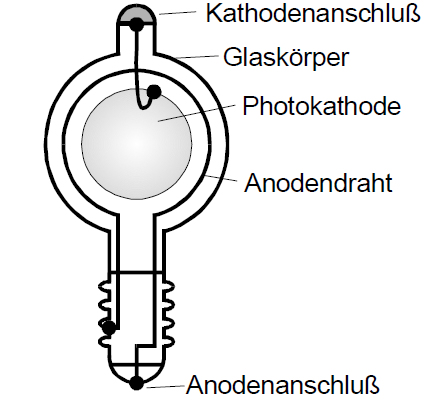
\includegraphics[width=0.4\textwidth]{Schematisch.png}
    \caption{Photozelle \cite{1}.}
    \label{fig:Schematisch}
\end{figure}
\noindent
Dabei ist entsprechend die Fläche der Kathode erheblich grö"ser als die der Anode um zu verhindern,
 dass auch aus der Kathode Photoelektronen austreten.
  Dies wird zusätzlich durch die Verwendung eines Materials untergedrückt, das eine erheblich höhere Austrittsarbeit als das Kathodenmaterial besitzt.\\

\subsection{Optischer Teil des Versuchsaufbaus}
Um monochromatisches Licht zur Bestrahlung zu erhalten werden die Lampen verwendet, die verschiedene wohlbekannte Spektrallinien emittieren.
 In diesem Fall ist dies eine Quecksilberdampflampe.\\
Um aus dem Licht monochromatisches Licht zu erhalten wird der in Abbildung \ref{fig:Optisch} dargstellten Aufbau verwendet.
Hierbei wird der Dispersionseffekt am Glasprisma verwendet, um die Spektrallinien räumlich voneinander zu trennen. 
\begin{figure}[H]
    \centering
    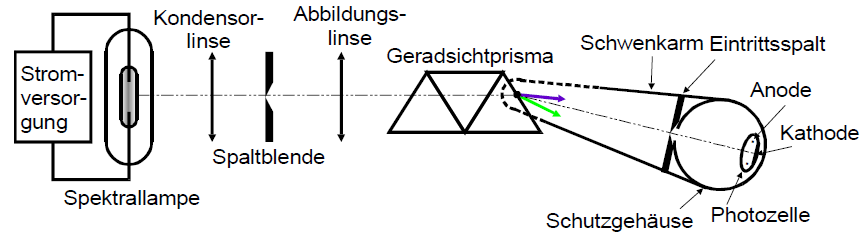
\includegraphics[width=0.9\textwidth]{Optisch.png}
    \caption{Versuchsaufbau \cite{1}.}
    \label{fig:Optisch}
\end{figure}
\noindent 
Die erste Linse wandelt das Licht in einen parallelen Strahlengang, der nachfolgende Spalt dient der Intensitätsregulierung und
 die zweite Linse bildet das Licht auf das Glasprisma ab. 
 Diese trennt die Spektrallinien auf und dann wird die Photozelle mit monochromatischem Licht beleuchtet.\\
Die Linsen sind dabei verschiebbar angeordnet, so dass   ihre Brennweite  entsprechend so einjustiert werden kann, 
dass eine scharfe Abbildung der Spektrallinien erhältet wird. Zudem muss darauf geachtet werden, 
dass die ausgewählte Spektrallinie möglichst intensiv ist um einen hohen Photostrom zu erzielen, der sich dann leichter nachzuweisen lässt.\\
Weiterhin wird eine rote Leuchtdiode für die rote Spektrallinie verwendet. Da diese natürlich bereits monochromatisches Licht aussendet entfüllt hierbei der optische Aufbau.

\subsection{Gegenfeldmethode}
Um nun Aussagen über die kinetische Energie der Elektronen zu treffen, wird die  Gegenfeldmethode (siehe Abbildung \ref{fig:Messapparatur}) verwendet.
\begin{figure}[H]
    \centering
    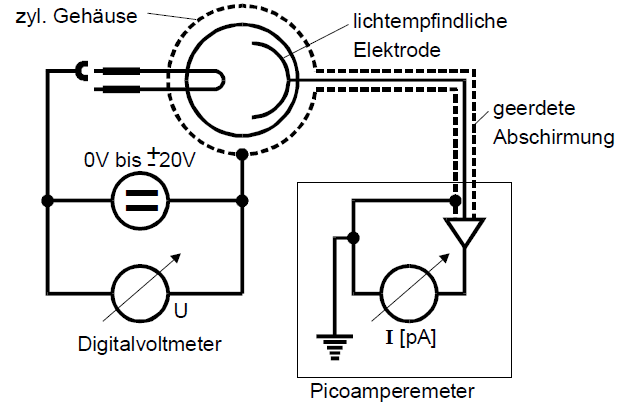
\includegraphics[width=0.7\textwidth]{Messapparatur.png}
    \caption{Elektrisches Schaltbild der Messapparatur \cite{1}.}
    \label{fig:Messapparatur}
\end{figure}
\noindent 
Die Elektronen werden aus einer Photokathode mittels Bestrahlung mit monochromatischem Licht ausgelöst.
Die ausgelösten Elektronen laufen gegen eine Gegenspannung $U$ an, die eine bremsende Wirkung auf sie ausübt.\\
Die  Gegenspannung wird nun auf einen Wert $U_g$ justiert, bei dem gerade keine Elektroden mehr an der Kathode ankommen.
Der Photostrom also verschwindet bei \( U=U_g\) wenn
 \begin{equation}
    e_0  \cdot U_{g}  = \frac{1}{2} m_0\, v_{\text{max}}^2\\
    \end{equation}
($e_0$: Elementarladung $e_0$, $m_0$: Ruhendemasse des Elektrons, $v_{\text{max}}$: Die Geschwindigkeit der schnellsten Elektronnen).\\
Somit haben die Elektronen genau ihre kinetische Energie in potentielle umgewandelt und es gilt
\begin{equation}
h \cdot \nu = e_0  \cdot U_{g}  + A_k.\\
\end{equation}
Praktisch verschwindet der Photostrom bereits bei \(U<U_g\) (siehe Abbildung \ref{fig:Photostrom}).
Zwischen dem Photostrom $I_\text{Ph}$ und der Bremmspannung $U$ besteht ein parabolischer Zusammenhang \(I_\text{Ph} \thicksim U^2 \).
\begin{figure}[H]
    \centering
    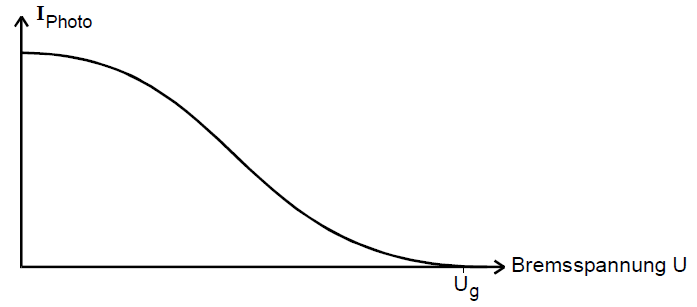
\includegraphics[width=0.7\textwidth]{Photostrom.png}
    \caption{Verhalten des Photostroms \cite{1}.}
    \label{fig:Photostrom}
\end{figure}
\noindent 
Deswegen besitzen die Photoelektronen nicht monoenergietische sondern eine Energieverteilung von 0 bis zu \(\dfrac{1}{2} m_0 v_{\text{max}}^2\).
Die Energie der Photoelektronen hängt von der Energie der Festkörperelektronen ab. Die Fermi-Dirac-Statistik  besagt,  
dass die Festkörperelektronen nicht allesamt die gleiche Energie besitzen, 
sondern eine Verteilung von 0 bis zur Fermi-Energie $\xi$.
Die Ursache vom Verhalten des Photostroms ist, dass nicht alle Photoelektronen die Annode erreichen, 
da Oberfläche der Anode viel zu klein ist und die Austrittsarbeit des Anodemetalls $A_A$ hoch ist.\\
Bei einer hohen Austrittsarbeit des Anodenmetalls $A_A$ müssen sich die ausgelösten Elektronen
gegen ein Gegenfeld bewegen, um auf die Anode zu treffen. Es wird ein beschleunigendes
Potential $U_b$ angelegt, um einen Photostrom zu erzeugen
\begin{align}
    h \nu + e_0 U_b \geq \ A_A \,.
\end{align}
\begin{figure}[H]
    \centering
    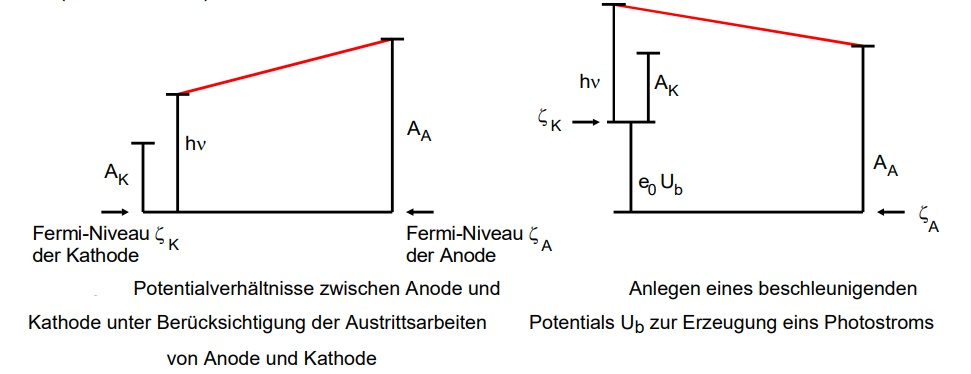
\includegraphics[width=1\textwidth]{Gegenfeld.jpg}
    \caption{Schematische Darstellung der Potentiale an Anode und Kathode \cite{1}.}
    \label{fig:Gegenfeld}
\end{figure}
\noindent 


\subsection{Messprogramm}
Zu Beginn wird  für verschiedene Wellenlänge des eingestrahlten Lichtes der
Elektronenstrom I in Abhängigkeit von der Spannung U der Photozelle gemessen. Damit
nur eine Spektrallinie pro Messung registriert wird, wird die Photodiode gedreht
und für die jeweilige Messung angepasst. Die Spannung wird in kleinen Schritten von 0
bis 2 V erhöht, bis kein Strom mehr zu messen ist. Daraufhin wird die Spannung bis -2
gesenkt.\\
Für den nächsten Aufgabenteil wird genauso vorgegangen wie im ersten Teil, aber für die Spektrallinie \(\lambda=579,1 \,\text{nm} \). 
Der Unterschied besteht darin, dass der Strom im Bezug der Spannung zwischen -20 und 20 V gemessen wird.\\
\label{sec:Durchführung}
